F�r das Modell \RN{2} war ein Konvergenzverhalten der Populationen zu beobachten. Diese konvergieren in Richtung eines station�ren Zustands. Sie werden auch als Ruhe- bzw. Gleichgewichtslagen $G$, des Lotka-Volterra-Modells, bezeichnet. Sie sind dadurch charakterisiert, dass keine zeitlichen Ver�nderungen der Zustandsvariablen mehr stattfinden \cite[S. 32]{lit:Foellinger1982}:

\begin{align*}
	\dot{x}_1 = 0, \qquad \dot{x}_2 = 0
\end{align*}

Damit folgt aus \autoref{eqn:grundl:x1} und \autoref{eqn:grundl:x2} \cite[S. 32]{lit:Foellinger1982}:

\begin{align}
	(a_1 - b_1 - c_1x_2)x_1 &= 0 
	\label{eqn:haupt:statx1} \\
	(a_2x_1 - b_2)x_2 &= 0
	\label{eqn:haupt:statx2}
\end{align}

Daraus ergibt sich zun�chst die triviale L�sung

\begin{align*}
	x_1 = 0, \qquad x_2 = 0
\end{align*}

in dem die R�uber sowie die Beute ausgestorben sind. Um den weiteren station�ren Zustand der Populationen zu bestimmen, m�ssen die beiden Ausdr�cke in den Klammern in \autoref{eqn:haupt:statx1} und \autoref{eqn:haupt:statx2} null werden \cite[S. 33]{lit:Foellinger1982}:

\begin{align}
	a_1 - b_1 - c_1x_2 &= 0
	\label{eqn:haupt:statx12} \\
	a_2x_1 - b_2 &= 0\
	\label{eqn:haupt:statx22} \
\end{align}

Daraus folgt, f�r die Zustandsvariablen $x_1$ und $x_2$, die Ruhelage $G$ \cite[S. 33]{lit:Foellinger1982}:

\begin{align}
	x_{1G} &= \frac{b_2}{a_2}
	\label{eqn:haupt:x1g} \\
	x_{2G} &= \frac{a_1 - b_1}{c_1}
	\label{eqn:haupt:x2g}
\end{align}

In dieser Gleichgewichtslage entspricht der Zuwachs an Beutetieren der Anzahl an durch die R�uber aufgezehrten Tiere. Ebenso bleibt die R�uberpopulation konstant. Da sich die Anzahl beider Populationen nicht �ndert, stellt die Gleichgewichtslage eine spezielle Trajektorie dar. Diese entspricht, wie in \autoref{img:haupt:phaseG} dargestellt, einem Punkt.

\begin{figure}
	\centering
	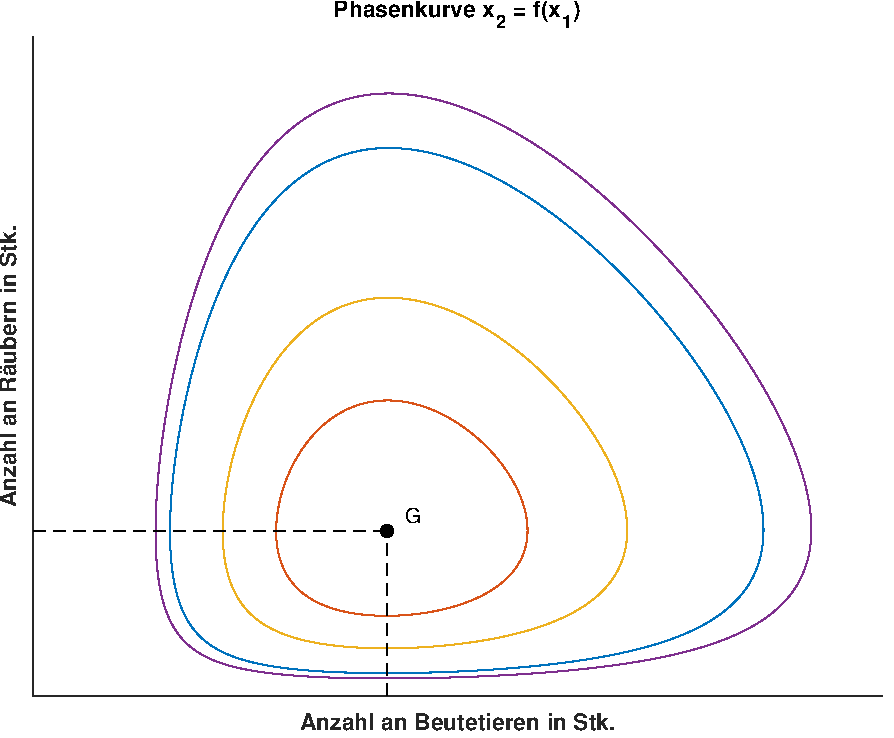
\includegraphics[width=0.6\linewidth,height=0.5\linewidth]{fig/exp/phaseG}
	\caption{Gleichgewichtslage in der Zustandsebene}
	\label{img:haupt:phaseG}
\end{figure}

Es ist anzumerken, dass die in \autoref{eqn:haupt:x1g} und \autoref{eqn:haupt:x2g} angegebenen Gleichgewichtslagen f�r $x_1$ und $x_2$ nicht von den Anfangspunkten abh�ngig sind. Diese Anfangspunkte bestimmen nur die entsprechende Trajektorie in der Zustandsebene. Die Ruhelage ist ausschlie�lich von den, in \autoref{sec:grundl:gl} genannten und beschriebenen, Faktoren $a_1, b_1, c_1, a_2,$ und $b_2$ abh�ngig. Diese beschreiben die entsprechenden Wechselwirkungen innerhalb und zwischen den Populationen. F�r die in \autoref{tab:haupt:param} gegebenen Werte, ergibt sich folgende Gleichgewichtslage:

\begin{align}
	x_{1G} &= \frac{b_2}{a_2} = \frac{0.1}{0.0002} = 500 \\
	x_{2G} &= \frac{(a_1 - b_1)}{c_1} = \frac{(0.05 - 0.02)}{0.0006} = 50
\end{align}

Eine M�glichkeit, die Gleichgewichtslage zu bestimmen, ist es diese numerisch zu approximieren. Hierzu wird in \autoref{lst:stat:code1} die Funktion $fsolve()$ verwendet. \autoref{eqn:haupt:statx12} und \autoref{eqn:haupt:statx22} werden, mit den entsprechenden Parametern $a_1, b_1, c_1, a_2$ und $b_2$, in einer anonymen Funktion gespeichert. Diese wird $fsolve()$ mit entsprechenden Startbedingungen �bergeben und anschlie�end die Gleichung $f = 0$ approximiert.

\begin{lstlisting}[style=Matlab-editor,caption={Verwenden von fsolve() f�r das numerische Bestimmen der Gleichgewichtslage},captionpos=b,label=lst:stat:code1,language=Matlab,basicstyle=\mlttfamily,numbers=none,frame=single,escapeinside={*@}{@*}]
% Parameter

% Beute / Hasen
a1 = 0.1; % Geburtenrate
b1 = 0.02; % Sterberate
c1 = 0.002; % Fressrate

% R�uber / F�chse
a2 = 0.0004; % Geburtenrate
b2 = 0.2; % Sterberate

% Deklarieren symbolischer Variablen
syms x1 x2
% Deklarieren der Gleichungen, um die Gleichgewichtslage zu bestimmen
f = @(x) [(a1 - b1 - c1*x(2));(a2*x(1) - b2)];
% Numerisches L�sen der Gleichungen mithilfe von vpasolve()
x = fsolve(f,[10,10])
\end{lstlisting}

Eine weitere M�glichkeit, die Gleichgewichtslage numerisch zu approximieren, ist mit der MATLAB Funktion $vpasolve()$ m�glich. In \autoref{lst:stat:code2} ist die Vorgehensweise hierzu exemplarisch dargestellt. In einem ersten Schritt werden hierbei die Parameter $a_1, b_1, c_1, a_2$ und $b_2$ deklariert und mit den in \autoref{tab:haupt:param} gegebenen Werten initialisiert. Anschlie�en werden, f�r die Zustandsvariablen $x_1$ und $x_2$, zwei symbolische Variablen mithilfe des \enquote{syms}-Befehls deklariert. Diese werden dazu verwendet, um \autoref{eqn:haupt:statx12} und \autoref{eqn:haupt:statx22}, unter Verwendung der symbolischen Variablen, in MATLAB zu definieren. Die definierten Gleichungen werden anschlie�end, mit der entsprechenden symbolischen Variablen, nach der die Gleichung aufgel�st werden soll, der Funktion $vpasolve()$ �bergeben. Diese approximiert numerisch N�herungswerte f�r $x_{1G}$ bzw. $x_{2G}$ und liefert die Ann�herungsl�sungen als R�ckgabewert.
\begin{lstlisting}[style=Matlab-editor,caption={Verwenden von vpasolve() f�r das numerische Bestimmen der Gleichgewichtslage},captionpos=b,label=lst:stat:code2,language=Matlab,basicstyle=\mlttfamily,numbers=none,frame=single,escapeinside={*@}{@*}]
% Parameter

% Beute / Hasen
a1 = 0.1; % Geburtenrate
b1 = 0.02; % Sterberate
c1 = 0.002; % Fressrate

% R�uber / F�chse
a2 = 0.0004; % Geburtenrate
b2 = 0.2; % Sterberate

% Deklarieren symbolischer Variablen
syms x1 x2
% Deklarieren der Gleichungen, um die Gleichgewichtslage zu bestimmen
eqnx1 = a1 - b1 - c1*x2 == 0;
eqnx2 = a2*x1 - b2 == 0;
% Numerisches L�sen der Gleichungen mithilfe von vpasolve()
% Erste Gleichung nach x2 aufl�sen
x2G = vpasolve(eqnx1, x2);
% Zweite Gleichung nach x1 aufl�sen
x1G = vpasolve(eqnx2, x1);
\end{lstlisting}

\FloatBarrier